% =============================================================================
% Section: MIRT discussion (MCQ track)
% Fully AI-drafted from the human outline heading ("MIRT Discussion", which only
% states the paper "highlights the promises and shortcomings of MIRT for MCQ").
% All prose is wrapped in \aiadd{...}; the section ends with an \aibullets{...}
% skeleton for a human rewrite. Every numeric claim traces to the CSV/README
% files listed below. Do not add uncited numbers.
%
% Expected preamble macros / packages (define in the main document if absent):
%   \usepackage{graphicx}   \usepackage{booktabs}   \usepackage{xcolor}
%   \newcommand{\aiadd}[1]{\textcolor{blue}{#1}}
%   \newcommand{\aibullets}[1]{\begingroup\color{blue}#1\endgroup} % group form wraps the itemize safely
%   \graphicspath{{figures/}}   % or copy figures next to the main .tex
%
% -----------------------------------------------------------------------------
% All \includegraphics calls use figures/<basename>. Copies of every basename are
% placed in BOTH _paper_build/figures/ and _paper_build/sections/figures/ so the
% path resolves whether the main .tex sits at the build root or in sections/.
% FIGURES REFERENCED (absolute source paths):
%   figures/filter_mechanism.png
%     <- /Users/arhant/Documents/EDLM/olmo-eval-full/AdaptiveTesting/Research/01_MCQ_ATLAS/data/link_failure_diagnosis/filter_mechanism.png
%   figures/bbh_diagnosis.png
%     <- /Users/arhant/Documents/EDLM/olmo-eval-full/AdaptiveTesting/Research/01_MCQ_ATLAS/data/link_failure_diagnosis/bbh_diagnosis.png
%   figures/mirt_vs_unidim_r.png
%     <- /Users/arhant/Documents/EDLM/olmo-eval-full/AdaptiveTesting/Research/01_MCQ_ATLAS/data/mirt_mcq/figures/mirt_vs_unidim_r.png
%   figures/latent_correlation_heatmap.png
%     <- /Users/arhant/Documents/EDLM/olmo-eval-full/AdaptiveTesting/Research/01_MCQ_ATLAS/data/mirt_mcq/figures/latent_correlation_heatmap.png
%   figures/bbh_dimensionality.png
%     <- /Users/arhant/Documents/EDLM/olmo-eval-full/AdaptiveTesting/Research/01_MCQ_ATLAS/data/mirt_within_benchmark/figures/bbh_dimensionality.png
%   figures/bbh_subtask_correlation_heatmap.png
%     <- /Users/arhant/Documents/EDLM/olmo-eval-full/AdaptiveTesting/Research/01_MCQ_ATLAS/data/mirt_within_benchmark/figures/bbh_subtask_correlation_heatmap.png
%   figures/bbh_cat_recovery.png
%     <- /Users/arhant/Documents/EDLM/olmo-eval-full/AdaptiveTesting/Research/01_MCQ_ATLAS/data/mirt_within_benchmark/figures/bbh_cat_recovery.png
%   figures/bbh_matched_budget.png
%     <- /Users/arhant/Documents/EDLM/olmo-eval-full/AdaptiveTesting/Research/01_MCQ_ATLAS/data/mirt_within_benchmark/figures/bbh_matched_budget.png
%
% DATA SOURCES (numbers in prose and tables):
%   .../data/link_failure_diagnosis/{README.md, diagnosis_summary.csv}
%   .../data/mirt_mcq/{README.md, mirt_mcq_results.csv, mirt_mcq_dimension_correlations.csv}
%   .../data/mirt_within_benchmark/{README.md, bbh_dimensionality.csv,
%       bbh_subtask_correlations.csv, bbh_cat_comparison.csv, bbh_cat_budget.csv}
%
% TODO(human): ATLAS is cited as the arXiv preprint (arXiv:2511.04689). The
%   authors' repo lists an ICML 2026 BibTeX and OpenReview shows an ICLR 2026
%   withdrawn submission; confirm the final venue and update refs/mirt_discussion.bib.
% =============================================================================

\section{MIRT discussion}
\label{sec:mirt-discussion}

\aiadd{The ATLAS pipeline we build on scores each MCQ benchmark with a single ability dimension~\cite{li2025atlas}. A natural question is whether one dimension is enough, or whether a multidimensional item response theory model (MIRT)~\cite{reckase2009mirt} recovers a benchmark's structure better. We answer this with three experiments on the OpenLM MCQ banks (ifeval, gpqa, math, bbh). Two findings frame the rest. First, a benchmark that looks like it cannot be scored is usually carrying broken items, not extra dimensions, so item hygiene has to come before any dimensionality claim. Second, once the items are clean, multidimensional modeling helps in proportion to how internally heterogeneous a benchmark is: it is worth the cost on a bundled suite like bbh, and it collapses back to the unidimensional model when a benchmark's skills are near-collinear.}

\subsection{Item quality comes before dimensionality}
\label{subsec:mirt-linkfailure}

\aiadd{Before reading a low correlation as evidence of multidimensionality, we checked whether it was an item-quality artifact. Calibration produces items with non-positive discrimination (\(a\le 0\)) when the fit fails or the response curve flips polarity. These items make more able models look less able, which scrambles the ability estimate. The MCQ banks carry many of them: \(51.4\%\) of fitted gpqa items, \(42.7\%\) of musr items, and \(31.2\%\) of bbh items have \(a\le 0\), against only \(1.9\%\) for math and \(4.5\%\) for ifeval (Table~\ref{tab:mirt-itemquality}).}

\aiadd{musr is the clean before-and-after case. On the same models and the same benchmark, dropping the \(43\%\) of junk items moves the CAT correlation with true accuracy from \(r=-0.036\) to \(r=0.746\). gpqa already used the canonical \(a>0\) loader, so its published CAT correlation never changed (\(r=0.737\)); the counterfactual makes the dependence visible anyway, because refitting full-bank ability recovery with the bad items included flips its sign from \(r=+0.32\) (filtered) to \(r=-0.07\) (unfiltered). math and ifeval have almost no bad items, so filtering does nothing to them, which is the control that rules out a benchmark-identity explanation. Neither gpqa nor musr is uninformative. The apparent link failure was a bank-hygiene bug, and panel (C) of Figure~\ref{fig:mirt-filter} shows its cause directly: a large mass of gpqa and musr items sits at \(a<0\).}

\begin{table}[tbp]
\centering
\small
\caption{\aiadd{Item quality, not benchmark identity, drives apparent link failure. Full-bank ability recovery (\(r\) between EAP ability and true accuracy) and CAT accuracy recovery, before and after the \(a>0\) filter. Source: \texttt{link\_failure\_diagnosis/diagnosis\_summary.csv}.}}
\label{tab:mirt-itemquality}
\begin{tabular}{l r r r r r}
\toprule
 & \(a\le 0\) & \multicolumn{2}{c}{full-bank \(r\)} & \multicolumn{2}{c}{CAT \(r\)} \\
\cmidrule(lr){3-4}\cmidrule(lr){5-6}
Benchmark & (\%) & unfilt. & filt. & pre & post \\
\midrule
math   &  1.9 & 0.83 & 0.84 & 0.878 & 0.878 \\
ifeval &  4.5 & 0.86 & 0.85 & 0.921 & 0.921 \\
bbh    & 31.2 & 0.69 & 0.86 & 0.753 & 0.674 \\
musr   & 42.7 & 0.49 & 0.62 & $-0.036$ & 0.746 \\
gpqa   & 51.4 & $-0.07$ & 0.32 & 0.737 & 0.737 \\
\bottomrule
\end{tabular}
\end{table}

\begin{figure}[tbp]
\centering

\includegraphics[width=\linewidth]{figures/filter_mechanism.png}
\caption{\aiadd{The \(a\le 0\) mechanism. (A) full-bank ability recovery, unfiltered versus filtered on the same target; (B) bank pollution per benchmark; (C) unfiltered discrimination distributions for gpqa and musr, with a large mass left of \(a=0\); (D) gpqa ability-versus-accuracy, unfiltered (\(r=-0.07\)) versus filtered (\(r=0.32\)).}}
\label{fig:mirt-filter}
\end{figure}

\aiadd{bbh is different. It stays weak after filtering (CAT \(r\approx 0.67\)), and this is not an item-quality problem: filtering lifts its full-bank ability recovery from \(r=0.69\) to \(r=0.86\), and its per-model score spread is healthy (score SD \(0.117\) on scored items), so low variance is not the issue either. The cause is early stopping. After filtering, bbh has the highest discriminations of any bank (median \(a=3.99\), against about \(1.4\) for gpqa and musr and about \(2.2\) for math). High-discrimination items collapse the posterior standard error quickly, so the CAT reaches the \(\mathrm{SE}\le 0.3\) target at its 8-item floor (mean \(8.2\) items, the fewest of any benchmark). Eight items badly under-sample a suite of roughly two dozen subtasks. Ability recovery error stays high (theta MAE \(0.68\)) and does not improve even at \(\mathrm{SE}\le 0.1\); predictions come out over-dispersed (prediction SD \(0.186\) against actual \(0.116\)) with the highest accuracy MAE of any benchmark (\(0.114\)). The full \(3{,}965\)-item bank recovers accuracy at \(r=0.86\), but the early-stopped CAT plateaus at \(r=0.67\), the largest full-bank-to-CAT drop we see (Figure~\ref{fig:mirt-bbhdiag}). The stopping rule is overconfident on a heterogeneous benchmark, which is exactly the failure the within-benchmark MIRT experiment (Section~\ref{subsec:mirt-within}) sets out to fix.}

\begin{figure}[tbp]
\centering

\includegraphics[width=\linewidth]{figures/bbh_diagnosis.png}
\caption{\aiadd{Why bbh stays weak after filtering. (1) score spread by benchmark (bbh is healthy, so variance is not the cause); (2) full-bank ability recovery versus CAT recovery with mean items (bbh drops the most and stops at about 8 items); (3) CAT prediction versus actual accuracy (bbh predictions are over-dispersed, highest MAE); (4) item p-value and discrimination median (bbh median \(a\approx 4\), an overconfident SE).}}
\label{fig:mirt-bbhdiag}
\end{figure}

\subsection{Across benchmarks: MIRT borrows strength across correlated skills}
\label{subsec:mirt-cross}

\aiadd{The first MIRT experiment pools the four MCQ banks into one between-item multidimensional model. Each benchmark is a latent dimension and the Q-matrix is simple benchmark membership. We calibrate a confirmatory two-parameter MIRT model, then run a single interleaved multidimensional CAT whose prior covariance is the estimated latent correlation matrix, so the ability update shares information across correlated dimensions~\cite{segall1996mat}. We compare that against four separate unidimensional CATs, one per benchmark. Calibration uses the \(1{,}101\) OpenLM models common to all four benchmarks (train \(991\), test \(110\)); after the \(a>0\) filter and subsampling, the dimensions hold \(150\) items each for ifeval, gpqa, and bbh, and \(77\) for math.}

\aiadd{Two caveats belong up front. We fit the model with the repository's numpy/scipy EM implementation of the marginal-maximum-likelihood M2PL~\cite{bock1981marginal}, not the R \texttt{mirt} package~\cite{chalmers2012mirt}, so the estimates are not identical to that reference implementation. And the math dimension enters thin, with only \(77\) items after pass-rate windowing and subsampling, so it is estimated less precisely than the others.}

\aiadd{At an \(\mathrm{SE}\le 0.3\) target, MIRT matches or beats the unidimensional baseline on accuracy recovery for all four benchmarks (Table~\ref{tab:mirt-cross}, Figure~\ref{fig:mirt-crossbar}). The largest gain is on math, where the unidimensional 2PL barely recovers accuracy (\(r=0.903\), MAE \(0.173\)) and MIRT reaches \(r=0.997\) with MAE \(0.020\). bbh improves from \(r=0.900\) to \(r=0.974\). gpqa barely moves (\(r=0.874\) to \(r=0.881\)), which fits the correlation structure below: gpqa shares the least with the other dimensions, so there is little correlated signal to borrow. This is the mechanism Segall described for multidimensional adaptive testing: a weak or near-floor dimension gains precision from its correlated neighbors.}

\begin{table}[tbp]
\centering
\small
\caption{\aiadd{Cross-benchmark accuracy recovery, MIRT versus per-benchmark unidimensional CAT, at two SE targets. Source: \texttt{mirt\_mcq/mirt\_mcq\_results.csv}.}}
\label{tab:mirt-cross}
\begin{tabular}{l l r r r r}
\toprule
 & & \multicolumn{2}{c}{MIRT} & \multicolumn{2}{c}{unidim} \\
\cmidrule(lr){3-4}\cmidrule(lr){5-6}
SE & Benchmark & \(r\) & MAE & \(r\) & MAE \\
\midrule
0.3 & ifeval & 0.985 & 0.036 & 0.962 & 0.053 \\
0.3 & gpqa   & 0.881 & 0.051 & 0.874 & 0.055 \\
0.3 & math   & 0.997 & 0.020 & 0.903 & 0.173 \\
0.3 & bbh    & 0.974 & 0.034 & 0.900 & 0.054 \\
\midrule
0.2 & ifeval & 0.990 & 0.032 & 0.976 & 0.051 \\
0.2 & gpqa   & 0.913 & 0.044 & 0.912 & 0.047 \\
0.2 & math   & 0.998 & 0.019 & 0.945 & 0.171 \\
0.2 & bbh    & 0.983 & 0.027 & 0.963 & 0.035 \\
\bottomrule
\end{tabular}
\end{table}

\begin{figure}[tbp]
\centering
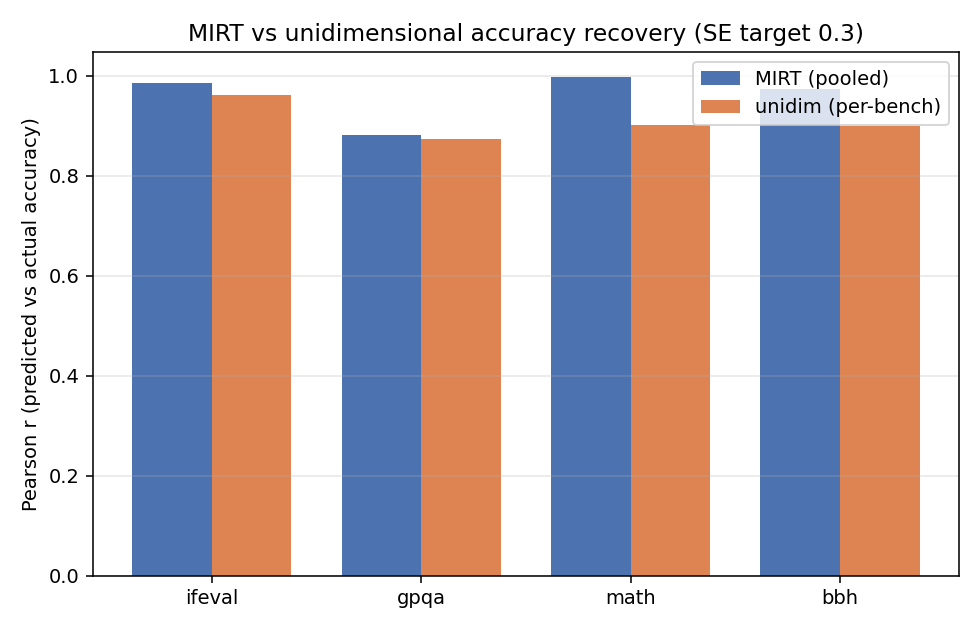
\includegraphics[width=\linewidth]{figures/mirt_vs_unidim_r.png}
\caption{\aiadd{MIRT (pooled) versus unidimensional (per-benchmark) accuracy recovery at \(\mathrm{SE}\le 0.3\). MIRT matches or beats the baseline on all four benchmarks, with the widest gap on math.}}
\label{fig:mirt-crossbar}
\end{figure}

\aiadd{The estimated inter-dimension correlations explain when borrowing helps (Table~\ref{tab:mirt-latent}, Figure~\ref{fig:mirt-latentheat}). Off-diagonal values range from \(0.09\) to \(0.76\) with a mean of \(0.44\). math and ifeval are the most correlated pair (\(0.76\)); gpqa and ifeval the least (\(0.09\)). None approach the \(0.8\) or higher that would mean the four skills collapse to a single factor, so the pooled bank is genuinely multidimensional and there is real, but uneven, strength to share.}

\begin{table}[tbp]
\centering
\small
\caption{\aiadd{Estimated latent inter-dimension correlations across the four MCQ benchmarks. Source: \texttt{mirt\_mcq/mirt\_mcq\_dimension\_correlations.csv}.}}
\label{tab:mirt-latent}
\begin{tabular}{l r r r r}
\toprule
 & ifeval & gpqa & math & bbh \\
\midrule
ifeval & 1.00 & 0.09 & 0.76 & 0.46 \\
gpqa   & 0.09 & 1.00 & 0.28 & 0.42 \\
math   & 0.76 & 0.28 & 1.00 & 0.61 \\
bbh    & 0.46 & 0.42 & 0.61 & 1.00 \\
\bottomrule
\end{tabular}
\end{table}

\begin{figure}[tbp]
\centering
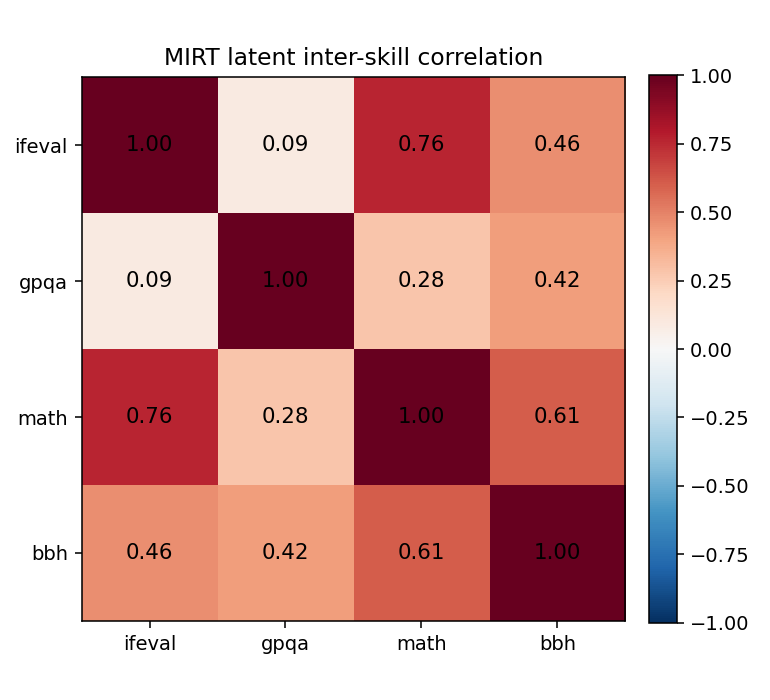
\includegraphics[width=0.9\linewidth]{figures/latent_correlation_heatmap.png}
\caption{\aiadd{Estimated latent correlations among the four MCQ dimensions. Moderate, mixed values (mean \(0.44\)) indicate genuine multidimensionality rather than a single collapsed factor.}}
\label{fig:mirt-latentheat}
\end{figure}

\aiadd{The gain has a cost. MIRT needs more total items to certify precision on every dimension, because the slowest dimension gates the single interleaved test. At \(\mathrm{SE}\le 0.3\), MIRT administers \(316.6\) items per model to reach the target on all four dimensions, against \(141.2\) for the sum of four separate unidimensional CATs; at \(\mathrm{SE}\le 0.2\) it is \(400.0\) against \(298.5\). The item counts in Table~\ref{tab:mirt-cross} mean different things for the two models (a unidimensional count is that benchmark's own test length, while a MIRT count is the pooled length when that dimension first hit target), so the per-model totals are the fair efficiency comparison. On this pooling, MIRT buys accuracy, not shorter tests.}

\subsection{Within bbh: heterogeneity is where MIRT pays off}
\label{subsec:mirt-within}

\aiadd{The second MIRT experiment fits the model inside a single benchmark, using bbh subtasks as latent dimensions, to ask whether bbh is internally multidimensional and whether modeling that recovers overall bbh accuracy better than a unidimensional CAT. The data are \(1{,}101\) OpenLM bbh models over \(3{,}759\) items after coverage filtering, with \(24\) subtasks that keep at least three usable items each (train \(991\), test \(110\)). A joint confirmatory M2PL over \(24\) dimensions is intractable for the fixed-grid EM, which needs \(\mathrm{grid}^{24}\) quadrature nodes, so we estimate the simple-structure latent correlation from per-subtask unidimensional EAP abilities and build the CAT bank from the per-subtask item parameters, with the estimated correlation matrix as the CAT prior covariance. This is a documented fallback, not the full joint fit.}

\aiadd{How many factors does bbh need? An exploratory MIRT fit on a balanced subsample (\(500\) models by \(288\) items) gives AIC and BIC that both keep dropping from \(k=1\) to \(k=6\), with no plateau at the largest \(k\) we could fit (Table~\ref{tab:mirt-dim}, Figure~\ref{fig:mirt-dim})~\cite{akaike1974aic,schwarz1978bic}. The one-factor model is the worst fit by a wide margin, which rules out treating bbh as unidimensional~\cite{hattie1985unidim}. So the effective dimensionality is at least six. One honest caveat: the \(k=5\) and \(k=6\) fits did not fully converge, so read six as a floor rather than a point estimate. Either way, the direction is clear and consistent with a suite of two dozen subtasks.}

\begin{table}[tbp]
\centering
\small
\caption{\aiadd{Exploratory dimensionality of bbh: AIC and BIC both keep falling through \(k=6\). Source: \texttt{mirt\_within\_benchmark/bbh\_dimensionality.csv}.}}
\label{tab:mirt-dim}
\begin{tabular}{r r r r c}
\toprule
factors \(k\) & loglik & AIC & BIC & converged \\
\midrule
1 & $-74168.2$ & 149488.4 & 155177.9 & yes \\
2 & $-67109.0$ & 135944.0 & 144468.4 & yes \\
3 & $-64096.7$ & 130491.3 & 141840.6 & yes \\
4 & $-60887.6$ & 124643.1 & 138807.6 & yes \\
5 & $-58547.5$ & 120530.9 & 137500.6 & no \\
6 & $-56672.7$ & 117347.4 & 137112.4 & no \\
\bottomrule
\end{tabular}
\end{table}

\begin{figure}[tbp]
\centering
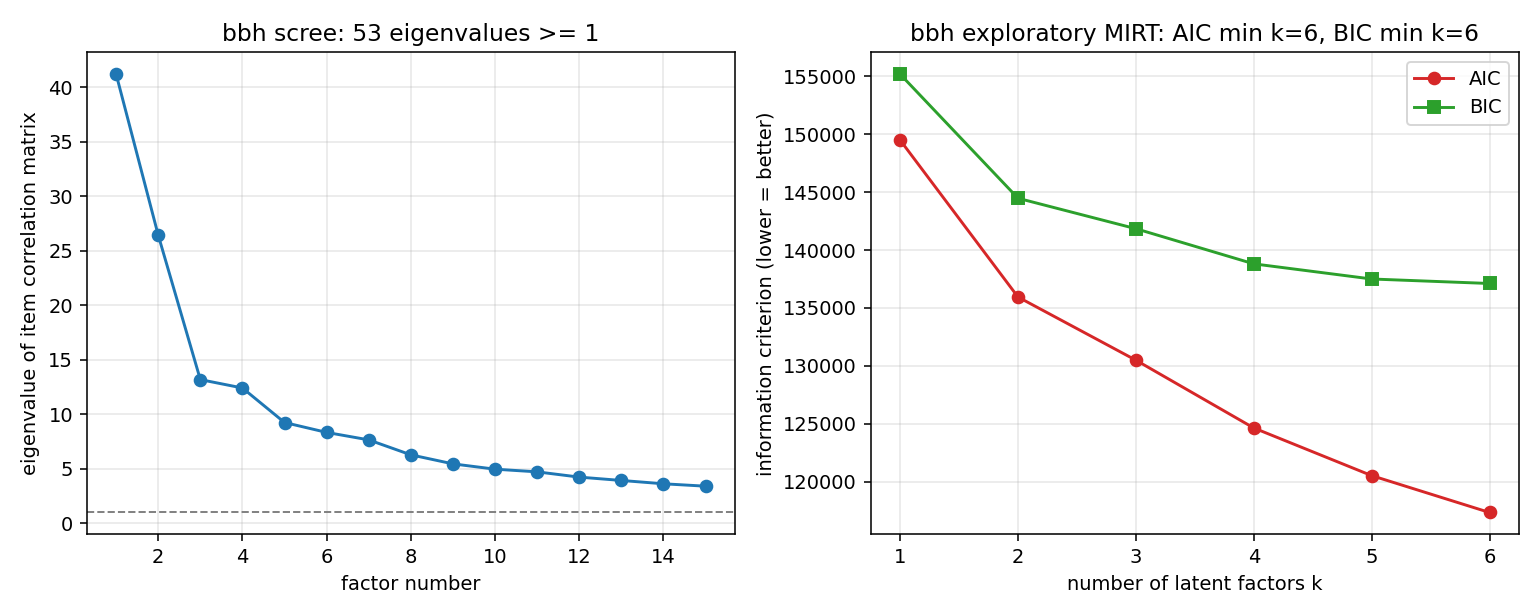
\includegraphics[width=\linewidth]{figures/bbh_dimensionality.png}
\caption{\aiadd{bbh dimensionality. AIC and BIC decrease from \(k=1\) through \(k=6\) without a plateau, and the eigenvalue scree has a long tail, so a single factor understates the benchmark's structure.}}
\label{fig:mirt-dim}
\end{figure}

\aiadd{The subtask correlation structure tells the same story from a different angle. The latent inter-subtask ability correlations have a mean of \(0.26\) and range from \(-0.63\) to \(0.89\) (mean \(0.27\) after disattenuating for reliability), shown in Figure~\ref{fig:mirt-subtaskheat}. The five- and seven-object logical-deduction subtasks correlate \(0.89\), while navigate and causal-judgement correlate \(-0.63\). A mean near \(0.26\) sits far below the \(0.8\) you would expect if one ability drove the whole suite, so bbh subtasks measure genuinely different skills.}

\begin{figure}[tbp]
\centering
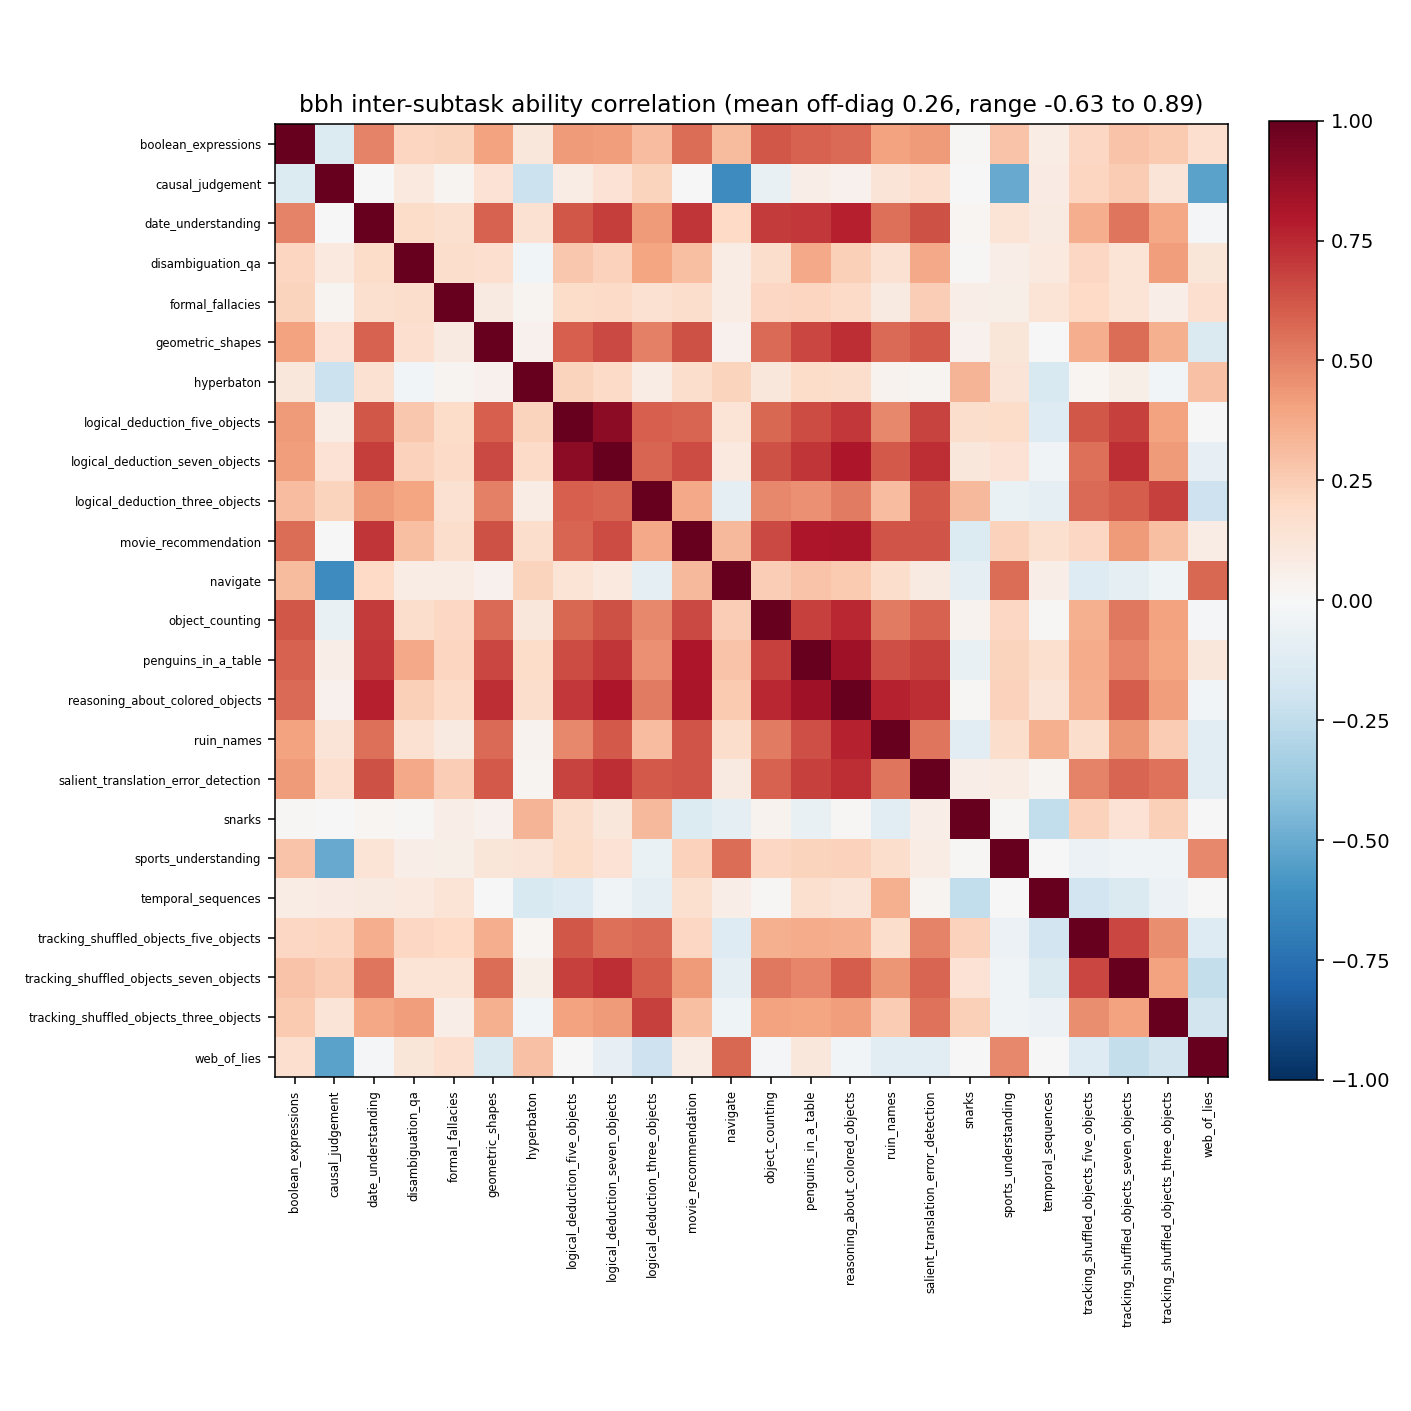
\includegraphics[width=0.9\linewidth]{figures/bbh_subtask_correlation_heatmap.png}
\caption{\aiadd{Latent ability correlations among \(24\) bbh subtasks (mean \(0.26\), range \(-0.63\) to \(0.89\)). The low mean confirms internal heterogeneity rather than one shared factor.}}
\label{fig:mirt-subtaskheat}
\end{figure}

\aiadd{Modeling that structure recovers overall bbh accuracy far better. At \(\mathrm{SE}\le 0.3\), the within-bbh MIRT CAT reaches \(r=0.973\) (MAE \(0.023\)) against the unidimensional CAT's \(r=0.845\) (MAE \(0.054\)) on the same held-out models (Table~\ref{tab:mirt-within}, Figure~\ref{fig:mirt-recovery}). The unidimensional CAT early-stops: its single ability estimate hits the target at a median of \(8\) items (mean \(13.4\)), the same under-sampling seen in the item-quality diagnosis. The MIRT CAT cannot early-stop on the whole heterogeneous suite, so it runs to the \(500\)-item cap. That is where the recovery gain comes from, and also why it costs many more items, which is what the matched-budget control isolates next.}

\begin{table}[tbp]
\centering
\small
\caption{\aiadd{Within-bbh MIRT versus unidimensional CAT, recovering overall bbh accuracy at the SE stopping rule. Source: \texttt{mirt\_within\_benchmark/bbh\_cat\_comparison.csv}.}}
\label{tab:mirt-within}
\begin{tabular}{l l r r r}
\toprule
SE & model & \(r\) & MAE & mean items \\
\midrule
0.3 & unidim & 0.845 & 0.054 & 13.4 \\
0.3 & MIRT   & 0.973 & 0.023 & 500.0 \\
0.2 & unidim & 0.855 & 0.055 & 37.3 \\
0.2 & MIRT   & 0.973 & 0.023 & 500.0 \\
\bottomrule
\end{tabular}
\end{table}

\begin{figure}[tbp]
\centering
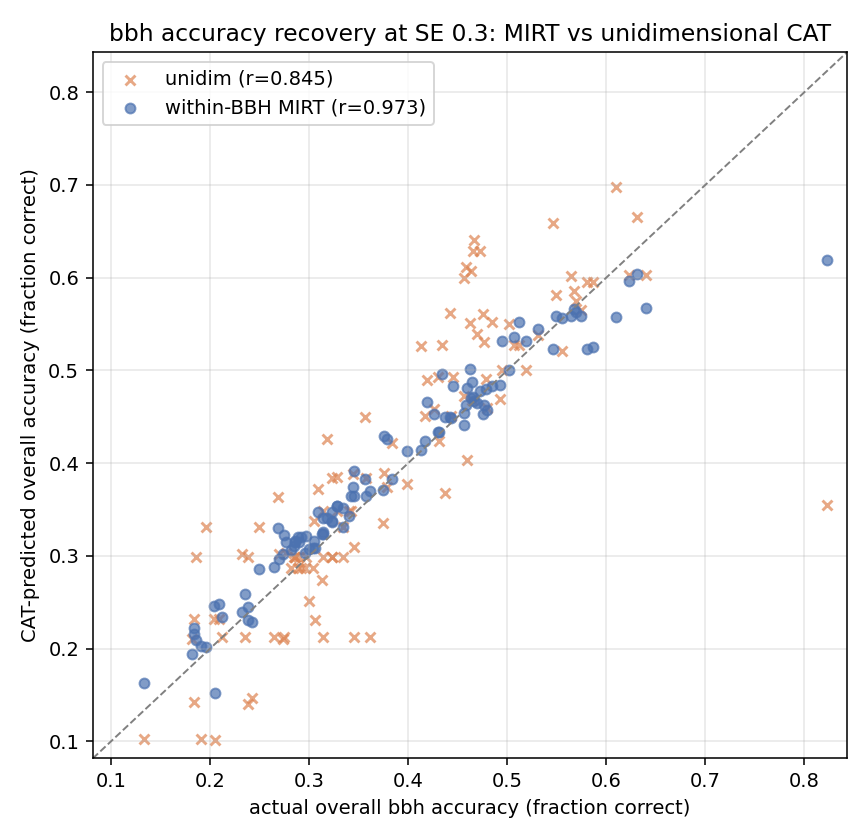
\includegraphics[width=0.9\linewidth]{figures/bbh_cat_recovery.png}
\caption{\aiadd{bbh accuracy recovery at \(\mathrm{SE}\le 0.3\). Within-bbh MIRT (\(r=0.973\)) tracks true accuracy far more tightly than the unidimensional CAT (\(r=0.845\)) on the same held-out models.}}
\label{fig:mirt-recovery}
\end{figure}

\aiadd{To separate modeling from test length, we force both CATs to the same number of items with no early stop (Table~\ref{tab:mirt-budget}, Figure~\ref{fig:mirt-budget}). MIRT wins at every budget: \(0.890\) against \(0.855\) at \(25\) items, \(0.924\) against \(0.861\) at \(50\), \(0.944\) against \(0.876\) at \(100\), \(0.960\) against \(0.892\) at \(200\), and \(0.969\) against \(0.915\) at \(400\). The gap is already there at \(25\) items and grows with budget, so the improvement comes from modeling the subtask structure, not from administering more items.}

\begin{table}[tbp]
\centering
\small
\caption{\aiadd{Matched item budget on bbh (no early stop). MIRT beats the unidimensional CAT at every fixed test length. Source: \texttt{mirt\_within\_benchmark/bbh\_cat\_budget.csv}.}}
\label{tab:mirt-budget}
\begin{tabular}{r r r r r}
\toprule
 & \multicolumn{2}{c}{\(r\)} & \multicolumn{2}{c}{MAE} \\
\cmidrule(lr){2-3}\cmidrule(lr){4-5}
items & unidim & MIRT & unidim & MIRT \\
\midrule
25  & 0.855 & 0.890 & 0.053 & 0.051 \\
50  & 0.861 & 0.924 & 0.053 & 0.040 \\
100 & 0.876 & 0.944 & 0.053 & 0.032 \\
200 & 0.892 & 0.960 & 0.051 & 0.028 \\
400 & 0.915 & 0.969 & 0.048 & 0.024 \\
\bottomrule
\end{tabular}
\end{table}

\begin{figure}[tbp]
\centering
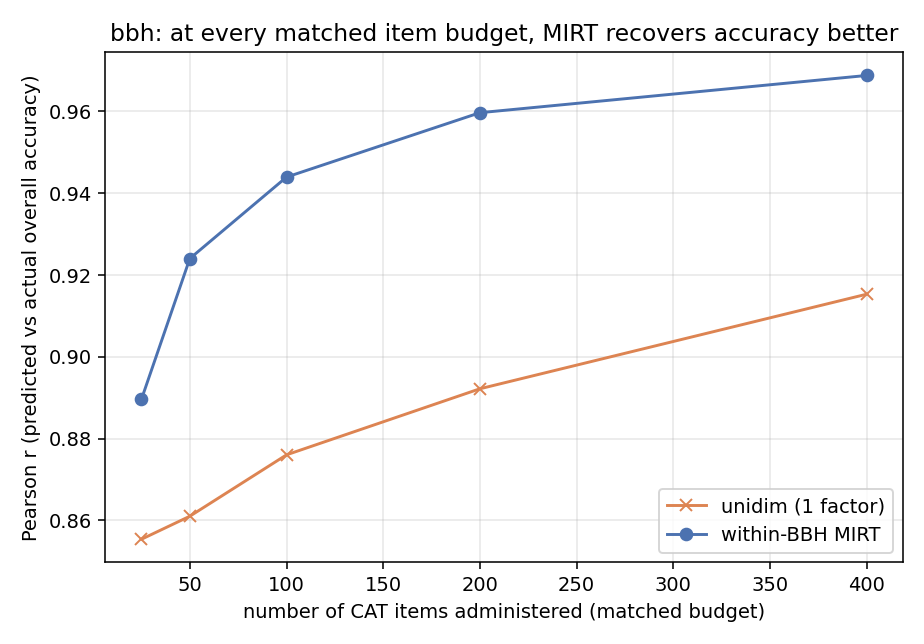
\includegraphics[width=0.9\linewidth]{figures/bbh_matched_budget.png}
\caption{\aiadd{Matched-budget recovery on bbh. At every fixed item count from \(25\) to \(400\), the within-bbh MIRT CAT recovers accuracy better than the unidimensional CAT.}}
\label{fig:mirt-budget}
\end{figure}

\subsection{Promises and shortcomings of MIRT for MCQ}
\label{subsec:mirt-tradeoffs}

\aiadd{The promise is real and it is specific. MIRT helps most when a benchmark is internally heterogeneous. Within bbh it lifts accuracy recovery from \(r=0.845\) to \(r=0.973\) at \(\mathrm{SE}\le 0.3\) and wins at every matched item budget. Across benchmarks it rescues a near-floor dimension by borrowing strength from correlated ones, taking math from \(r=0.903\) to \(r=0.997\). It also diagnoses and repairs a failure mode of unidimensional CAT: a single ability estimate can collapse on a handful of high-discrimination items and quit before it has sampled the suite, which is precisely what makes bbh look weak under a unidimensional 3PL.}

\aiadd{The shortcomings are just as concrete. When latent dimensions are near-collinear, the multidimensional model reduces to the unidimensional one and adds little for the extra machinery; and where a dimension shares little with its neighbors, as gpqa does here, there is not much strength to borrow either. MIRT also costs more items to certify precision on every dimension, because the slowest dimension gates the interleaved test (\(316.6\) against \(141.2\) items across benchmarks at \(\mathrm{SE}\le 0.3\), and the \(500\)-item cap within bbh). The joint model is computationally heavy: a full confirmatory fit over many dimensions is intractable for the fixed-grid EM, which forced the simple-structure fallback. Two estimation caveats carry through: our fits use a numpy/scipy EM rather than the R \texttt{mirt} package~\cite{chalmers2012mirt}, and the largest exploratory fits (\(k=5,6\)) did not fully converge. Finally, item hygiene is a precondition, not an option. The \(a>0\) filter from Section~\ref{subsec:mirt-linkfailure} has to run first, or the multidimensional bank inherits the same reversed-curve items that break the unidimensional one.}

\aiadd{The practical reading is that MIRT for MCQ pays off in proportion to a benchmark's internal heterogeneity. On a bundled suite like bbh it is worth the extra items and compute. On a coherent benchmark whose skills are near-collinear, it collapses to the unidimensional model, and the simpler 3PL CAT is the better default.}

% ---- Human-rewritable skeleton (key claims, each traceable to a CSV/README) ----
\aibullets{
\begin{itemize}
  \item Item quality first: non-positive discrimination items (gpqa \(51\%\), musr \(43\%\), bbh \(31\%\)) caused apparent link failure; musr CAT \(r=-0.036\to 0.746\) after filtering, gpqa full-bank recovery sign-flips \(-0.07\to +0.32\), and math/ifeval are unaffected (control).
  \item bbh is the genuinely weak case for a different reason: inflated discriminations (median \(a\approx 4\)) trigger an 8-item early stop that under-samples about two dozen subtasks; full-bank ability recovers accuracy at \(r=0.86\) but the early-stopped CAT plateaus at \(r=0.67\).
  \item Cross-benchmark MIRT matches or beats unidimensional recovery on 4/4 at \(\mathrm{SE}\le 0.3\); biggest gain on math (\(0.903\to 0.997\)), essentially flat on gpqa (the least-correlated dimension); latent correlations span \(0.09\) to \(0.76\), mean \(0.44\), so no single collapsed factor.
  \item Cost of the pooled MIRT: more total items to certify all dimensions (\(316.6\) vs \(141.2\) at \(\mathrm{SE}\le 0.3\)), because the slowest dimension gates the interleaved test.
  \item Within bbh: effective dimensionality at least 6 (AIC and BIC drop through \(k=6\); \(k=5,6\) not fully converged); subtask ability correlation mean \(0.26\) (range \(-0.63\) to \(0.89\)); MIRT CAT \(r=0.973\) vs unidim \(0.845\) at \(\mathrm{SE}\le 0.3\); MIRT wins at every matched budget (\(25\): \(0.890\) vs \(0.855\); \(400\): \(0.969\) vs \(0.915\)).
  \item Promise: MIRT helps in proportion to internal heterogeneity, borrows strength across correlated skills, and fixes the unidimensional early-stop under-sampling.
  \item Shortcoming: near-collinear dimensions collapse to unidimensional; certifying every dimension needs more items; the joint fit is intractable at high dimension (simple-structure fallback); fits use a numpy/scipy EM, not R \texttt{mirt}; and the \(a>0\) hygiene step is required first.
  \item Caveats to state plainly for a reviewer: numpy/scipy EM M2PL rather than R \texttt{mirt}; the math dimension is thin (\(77\) items after pass-rate windowing and subsampling); exploratory \(k=5,6\) did not fully converge; the within-bbh MIRT CAT hits a \(500\)-item cap rather than early-stopping.
\end{itemize}
}
